\documentclass[a4paper,11pt]{article}
\usepackage[utf8]{inputenc}
\usepackage[colorinlistoftodos, textwidth=2cm, shadow]{todonotes}
\usepackage{listings}
\usepackage{appendix}
\usepackage[colorlinks=true,linkcolor=blue]{hyperref}
\usepackage[section]{placeins}
\lstset{
	language=C
  }

\topmargin 0pt
\advance \topmargin by -\headheight
\advance \topmargin by -\headsep
\textheight 8.9in
\oddsidemargin 0pt
\evensidemargin \oddsidemargin
\marginparwidth 0.5in
\textwidth 6.5in
\parindent 0in
\parskip 1.5ex

\title{\emph{dsinf}: Source Based Data Structure Inference}
\author{Aleksander Balicki}
\date{\today}

\begin{document}

\vfill

\maketitle

\begin{abstract}

    When you need to store data in a data structure, most of popular languages
    today already have libraries with convenience data structures implemented.
    Programmers just have to be taught when to use a particular data structure. Some of
    the cases of choosing the right data structure look sufficiently easy, so a
    program could do it automatically. This work describes the \emph{dsinf} project,
    an analysis framework for inferring the best data structure matching the task,
    based on the program's source code in C language. \emph{dsinf} analyses the 
    uses of data structures throughout the program and suggests the fastest one.     
    To further enhance the quality of the suggestion, it uses profiler data.

\end{abstract}

\pagebreak

\tableofcontents

\vfill

\section{Introduction} \label{sec:intro}
	In computer science, a data structure is a particular way of storing and organizing data in a computer so that
	it can be used efficiently\cite{Wids}.

	The interface of a data structure is a set of operation that you can perform on a data structure and some
	semantics of those operations.

	The implementation of a data structure is a realization of some data structure interface in some programming
	language, that is consistent with the semantics.

	There is a lot different known types of data structures:
	\begin{itemize}
		\item Map/Associative array/Dictionary is a data structure for storing $(key,\;value)$ pairs, it allows
			insertion, deletion, modification and lookup,
		\item multimap is the same as Map, but with the possibility of storing multiple values for a one key,
		\item list is a data structure for storing ordered sets of values,
		\item set is a data structure for storing unordered sets of values,
		\item multiset is the same as Set, but with the possibility of storing multiple objects that are equal
			under some equivalence relation,
		\item queue is a data structure implementing operations for queuing and dequeuing elements,
		\item deque is a queue, where you can add and remove elements from both ends as opposed to one,
		\item stack is a data structure implementing operations for putting something on the top of the stack or
			removing the top element from it,
		\item priority queue is like a regular queue, but each element has a priority associated with it, which
			is used for ordered dequeuing of the elements,
		\item string is a data structure for storing text,
		\item tree is a data structure, to hold some tree-like hierarchical structure,
		\item graph is a data structure, to store elements and a relation on those elements,
		\item others, which usually are a modification or a mix of previous ones.
	\end{itemize}

	The different implementation of those data structures make it possible, that specific operations run time is
	lower than the others. So there is no data structure perfect for all the tasks.

	\subsection{What is dsinf?} \label{sub:intro}

		dsinf is a source code analyzer. It works by analyzing specially prepared C code. That C code, for every
		instance of a data structure, uses a type defined in the dsinf library. This type is called a data
		structure wildcard. The type represents a data structure with the most general interface, i.e. a set union
		of interfaces of all data structures available in the dsinf framework. It connects the data structures
		and operations performed on them and then reasons about which of the available data structure
		implementations would be best for the instances of data structure wildcards in your code, finally (if
		possible) choosing the best matches and printing them out or linking them to your code to create a
		working binary.

		The above analysis now works after compiler C code preprocessing (using CPP or a preprocessor included in a C compiler), before the actual compilation. In the future it can be
		pushed to the phase between compilation and linking as described in \autoref{sec:future}.

		The analysis process uses asymptotic complexity for data structure comparison. The process can also be
		modified by providing some source code annotations or you can use test data to tailor your data
		structure as described in \autoref{sub:importance}.

		The idea of the framework is to provide a data structure, that when used is always good enough. Due to
		unsolvability of the general case of the problem, the effect always will be worse than a hand tailored
		data structure to your task, but can save up some time (both programming time and execution time) if the
        time is an important factor. To reiterate, using dsinf for the most critical bottleneck of your
		application probably isn't a good idea.

	\subsection{Comparing to a database} \label{sub:database}
        There's already a mature solution for storing data and querying it in an efficient way --- databases.
		The main difference between dsinf and a database is that a database has to implement all the operations
		for all the possible SQL queries, including some crosschecks, counting, summations, extremal elements
		and with dsinf your data structure implementation doesn't have to be ready for all the possible SQL
		queries that can be constructed, but only the ones you used in your source code, which enables it to
		potentially gain some performance over a database, both in space and time complexity.

	\subsection{Comparing to class clusters} \label{sub:classcluster}
		A class cluster is an architecture that groups a number of private, concrete subclasses under a public,
		abstract superclass. The grouping of classes in this way provides a simplified interface to the user,
		who sees only the publicly visible architecture. Behind the scenes, though, the abstract class is
		calling up the private subclass most suited for performing a particular task\cite{AppleCC}. One could
		have an object representing e.g. an array, and have a lot of different private implementations for it, like
		large, sparse arrays, or arrays with sizes known at compile time and optimize operations for those
		cases. The downside of such method is that you can alternate between the data structure representations
		that need a lot of time to transform into each other. dsinf knows exactly what operations can occur and
		tailors the data structure to the operations that will happen.

	\subsection{C API}
        The framework detects specific C functions in the source code and bases the inference on them. Now we define
        what are those functions. The first API version is on \autoref{fig:C-api-v1}.

        \begin{figure}[h!]
            \lstinputlisting{thesis-pics/ds1.h}

            \caption{The simplified dsinf C API}

            \label{fig:C-api-v1}
        \end{figure}

        There is a problem with \autoref{fig:C-api-v1} API. If there's an
        operation on a data structure that is asymptoticly faster than the
        speed of a lookup of an element, it's impossible to obtain in the
        desired time with this API. For example, a balanced search tree
        that guarantees $O(log n)$ lookups, with a linked list of all the
        elements (like in \autoref{sec:gdsm:le}) to enhance the speed of the
        successor and predecessor operations to $O(1)$. Defining a successor
        function using this API convention, it would look like this:

        \begin{lstlisting}
dstype successor_d(ds, dstype);
        \end{lstlisting}

        The problem with this function is that it doesn't take a pointer to the element in a data structure, so it has
        to actually find the value given in the actual parameter of the function, and then compute the successor in
        $O(1)$, but the search takes $O(log n)$, so the whole operation takes $O(log n)$, which is bad.

        To fix this we declare a new type for an data structure element. The type encompasses a pointer to the place in
        the data structure. The search can be started from this pointer, so there is no need to waste time on finding the element.

        The second version of the API is on \autoref{fig:C-api-v2}. It's updated to use the $dselem$ struct. We use the pointer value instead of the simple value like before.

        \begin{figure}[h!]
            \lstinputlisting{thesis-pics/ds2.h}
            \caption{The dsinf C API}

            \label{fig:C-api-v2}
        \end{figure}

        The following code examples will sometimes use \autoref{fig:C-api-v1} API convention for simplicity.

\section{Data structure inference}

	\subsection{Comparison of the complexities}

		If we want to find the best possible data structure for a task, we have to define some kind of ordering
		on the data structures, so we can judge which structures are better than others. Here we want to compare the
		asymptotic complexities of operations on data structures. When trying to define such ordering, we
		encounter a problem.  We can't do it for the general case, because the complexity of an operation
        can be described by arbitrary functions and a comparison of asymptotic complexities is complicated.

		Asymptotic complexity of an operation is stored as a pair of type:

		\begin{eqnarray}
			AsymptoticalComplexity = Int \times Int,
		\end{eqnarray}

		where

		\begin{eqnarray} \label{eqn:linlog}
			(k, \; l) \; means \; O(n^k \log^l{ n}).
		\end{eqnarray}

		The reason to choose such a type is that it's easier to compare than the general case (we can do a
		lexicographical comparison of the two numbers) and it distinguishes most of the data structure operation
		complexities.

		Sometimes we have to use some qualified complexities:

		\begin{eqnarray}
			ComplexityType = \{ Normal, \; Amortized, \; Amortized \;Expected, \; Expected \}
		\end{eqnarray}

		The overall complexity can be seen as a type:

		\begin{eqnarray}
			Complexity = AsymptoticalComplexity \times ComplexityType
		\end{eqnarray}

		Here we can also use a lexicographical comparison, but we have to say that

		\begin{eqnarray}
			Amortized > Normal,\\
			Expected > Amortized,\\
			Amortized \; Expected > Expected
		\end{eqnarray}

		and that $>$ is transitive.

		The ordering is done in such way, because normal complexity of $O(f(n))$ guarantees that no operation
		will exceed that time multiplied by a constant. Amortized is worse, because here, we can only guarantee
		that $n$ consecutive operations will have the average time $O(f(n))$, but single operations can spike
		heavily. Expected is worse than amortized, because here we can only have some probability of achieving
		the mentioned complexity for an operation and there's no bound on the number of spikes, which were under
		control in an amortized complexity.

		We also always choose the smallest asymptotic-complexity-wise complexity.  For example, we have a search
		operation on a splay tree. It's $O(n)$, but $O(\log n)$ amortized, so it's represented as
		$((0,1),Amortized)$.

	\subsection{Choosing the best data structure} \label{sec:choose-ds}

		We define a set $DataStructureOperation$. We can further extend this set, but for now assume that

		\begin{eqnarray}
			DataStructureOperation = \{Insert, \; Update, \; Delete, \; FindMax,\; DeleteMax, \; \dots\}.
		\end{eqnarray}

		Each of the $DataStructureOperation$ elements symbolizes an operation you can accomplish on a data
		structure.

		The type

		\begin{equation}\label{data-structure-type}
			DataStructure = DataStructureOperation \rightarrow Complexity
		\end{equation}

		represents a data structure $ds$ and all of the operations implemented for it, with their complexities, as a
		partial function $f$ from DataStructureOperation to Complexities. It represents some implementation of a
		data structure, where existing arguments of $f$ are the operations, which are possible to accomplish on
		$ds$, and the value of the function represents asymptotic speed of the operation. For example
		\autoref{tab:rbt} presents such representation for Red-Black Trees.

		\begin{table}[h!]
			\centering
			\begin{tabular}{|l|l|}
				\hline
				\multicolumn{2}{|c|}{Red-Black Trees} \\
				\hline
				Operation & Complexity \\
				\hline
				Insert 	        & $O(log \; n)$ \\
				Update          & $O(log \; n)$ \\
				Delete	        & $O(log \; n)$ \\
				Find Max 	& $O(log \; n)$/$O(1)$\\
				Delete Max	& $O(log \; n)$ \\
				Search 		& $O(log \; n)$ \\
				Successor 	& $O(log \; n)$/$O(1)$\\
				\hline
			\end{tabular}
			\caption{A table showing the representation of Red-Black trees; complexity varies on
			implementation, speed-up technique described in \autoref{sub:gdsm}}
			\label{tab:rbt}
		\end{table}

		When trying to find the best suited data structure for a given program $P$, we look for data structure
		uses in $P$. Let

		\begin{equation} \label{dsu-type}
			DSU(P) :: [P(DataStructureOperation)]
		\end{equation}

		be a set of groups of data structure operations. One group represents operations on one persistent
        data structure identity in the source code of $P$.

		For every $ds \in DSU(P)$, we define a parametrized comparison operator for data structures $<_{ds}$
		defined as:

		\begin{center}

			\begin{equation}
				d_1 <_{ds} d_2
			\end{equation}

			$\Updownarrow$

			\begin{equation} \label{data-structure-order}
|\{(o, c_1) \in d_1 | o \in ds \wedge o \texttt{ used in $P$} \wedge (o,c_2) \in d_2 \wedge c_1 < c_2 \}| < 0.5 *
 |\{o \in ds | o \texttt{ used in $P$} \}|
			\end{equation}

		\end{center}

        From data structures $d_1$ and $d_2$ we compare costs ($c_1$, $c_2$ respectively) of all the operations.

		If a data structure implements more operations "faster" then that structure is higher in the order defined
        in \autoref{data-structure-order}.

		For a fixed P, we have a preorder on data structures induced by $<_{ds}$ and we can sort data structures
		available to the framework using this order. The maximum element is the best data structure
		implementation for the persistent data structure identity.

	\subsection{Collecting the program data} \label{dsu-definition}

		In \autoref{dsu-type} the type of the $DSU()$ operation was mentioned, this section shows, how $DSU()$ is
		defined. We're not considering the problem of 2 different variables having the same name and/or shadowing each
        other, to evade this we can just rename each variable to an UUID, and then remember the mapping for nicer
        output.

		Let $DSOPS(P) :: [(VariableName, DataStructureOperation)]$ be the union of:
		\begin{enumerate}

			\item \label{it:global} $\{(g, o)\; |\; g \texttt{ is a global data structure variable in $P$ }
				\wedge \\ o \texttt{ is an operation performed on $g$, somewhere in $P$ } \}$

			\item \label{it:auto} $\{(d, o)\; |\; d \texttt{ is a data structure declared somewhere } \\
				\texttt{ in a body of a function $f$ in $P$ } \wedge \\ o \texttt{ is an operation
				performed on $d$, somewhere in $f$ } \}$

			\item \label{it:param} $\{(p, o)\; |\; p \texttt{ is a formal parameter of data structure type,}
				\\ \texttt{of a function $f$ in $P$ } \wedge \\ o \texttt{ is an operation performed on
				$p$, somewhere in $f$ } \}$

		\end{enumerate}

        \begin{figure}[h]
            \lstinputlisting{thesis-pics/collecting_global.c}

            \caption{Shows sn example of the global variables collection rule}

            \label{fig:global-collection-rule}
        \end{figure}
        \begin{figure}[h]
            \lstinputlisting{thesis-pics/collecting_declared.c}
            \caption{Shows sn example of the declared variables collection rule}

            \label{fig:declared-collection-rule}
        \end{figure}
        \begin{figure}[h]
            \lstinputlisting{thesis-pics/collecting_function.c}

            \caption{Shows sn example of the function parameters collection rule}

            \label{fig:parameter-collection-rule}
        \end{figure}

        \clearpage


		We want to group the elements in $DSOPS(P)$ to detect the persistent identities \cite{Okasaki} of
		data structures, meaning that in one group, there will be data structure operations conducted on one
		data structure from its allocation, to deallocation or the end of the program, counting in passing the structure as a
		parameter to another function or copying the pointer to the structure.

		To group the operations:
		\begin{itemize}

            \item \textbf{Persistent Identities} - for every two pairs $(d_1, o_1)$ and $(d_2, o_2)$ created using
                \autoref{it:global} or \autoref{it:auto}, we put them in the same group if $d_1 = d_2$.

            \item \textbf{Function calls} - for every pair $(p, o_1)$ that was created by using \autoref{it:param}
                from function $f$, which was called with the actual data structure parameter $d$ as the formal parameter
                $p$, we put $o_1$ into the group of operations on $d$.

            \item \textbf{Copy propagation} - for every $(do, o_1)$ and $(dc, o_2)$, where the $dc$ variable was
                obtained by copying the value of the variable $do$, we put $o_1$ and $o_2$ in the same group.

            \item \textbf{Uniqueness} - for every group, we delete repeating elements

		\end{itemize}

        \begin{figure}[h]
            \lstinputlisting{thesis-pics/function-call-grouping.c}

            \caption{An example of using the function call grouping rule}

            \label{fig:function-call-grouping}
        \end{figure}

        \clearpage

		$DSU(P)$ is the list of those groups. After this operation, each group has operations performed on the
		same persistent identity of a data structure. For every such group we find the best matching data
		structure like shown in \autoref{sec:choose-ds}.


\pagebreak

\section{Extensions of the idea}

	\subsection{Second extremal element}

		If we want to find the maximal element in a heap, we just look it up in $O(1)$, that's what heaps are
		for.  If we want to find the minimal element we can modify the heap, for it to use an order, which would
		allow us to lookup the minimal element in $O(1)$.  What happens if we want to find the max and the min
		element in the duration of one program?  How to modify our framework to handle this kind of situations?

		\begin{eqnarray*}
			DataStructureOperation = \{\dots, \; FindFirstExtremalElement,\\
			DeleteFirstExtremalElement,\\
			FindSecondExtremalElement,\\
			DeleteSecondExtremalElement\}.
		\end{eqnarray*}

        Now we can add two complexity costs to the data structure definition. We always try to map the first extremal
        element to the kind of element that is used more. We can always reverse the order, so the cheaper one can be
        used primarily, and the more expensive one in situations when we need both types of extremal elements.

	\subsection{Importance of operations} \label{sub:importance}

		Detecting the importance of a single data structure operation is an important problem, because a lot of
		programs will fall into a class where compile-time data structure selection is undecidable. The
        program in \autoref{fig:undecidable} shows that the problem of compile-time deciding on the best data structure
        is impossible to solve.

        \begin{figure}[!h]
			\lstinputlisting{thesis-pics/undecidable.c}

			\caption{An example of the problem of choosing the fastest data structure for a program being
			undecidable, user interaction}

			\label{fig:undecidable}
		\end{figure}

		In \autoref{fig:undecidable}, the best data structure is depending on the user input, which is not known at
		compile time. If we analyze it as is, it will decide basing on the information, that every operation is
		used, so the final data structure won't be specific to the task, but just average at everything.

		The code that is not totally dependent on the user input can also cause problems to analyze.

        \begin{figure}[!h]
			\lstinputlisting{thesis-pics/weighted-instructions.c}

			\caption{An example of the problem of choosing the fastest data structure for a program being hard to
            analyze, no user interaction}

			\label{fig:hard-no-user}
		\end{figure}

		In \autoref{fig:hard-no-user} we see a very costly instruction used only once
		($delete\_max\_d$), and a few instructions ($insert$, $search$) run in a loop for a few million times.
		To anyone that knows program complexities it's obvious that this one heavy instruction doesn't affect
		the execution time of the whole program, yet the framework at the current state treats those
		instructions equally and will probably choose something like Red-Black Trees, to minimize the time of
		the $delete\_max\_d$, instead of ignoring its cost and using a very fast Hashtable.

        We can formally show, that the problem of choosing the fastest data structure is undecidable, by showing that
        it's not easier than the halting problem. In \autoref{fig:undecidable-no-user} we run the $delete\_max\_d$ only
        if a turing machine that we defined accepts an input, so we don't know if we should choose a data structure that
        implements $delete\_max\_d$ fast, or just ignore it, because it won't ever be used because of the machine not
        stopping the computation.

        \begin{figure}
			\lstinputlisting{thesis-pics/turing-machine.c}

			\caption{An example formally showing the undecidability of the problem, no user interaction}

			\label{fig:undecidable-no-user}
		\end{figure}

		\subsubsection{Code pragmas} \label{sec:pragmas}

			A possible solution to this problem is to let the programmer add code pragmas to his source
			code, so he decides how important an instruction is in relation to other instructions and then
			the framework makes use of those values in choosing the data structure.

            \begin{figure}[!h]
				\lstinputlisting{thesis-pics/code-pragmas.c}

				\caption{Source code with pragmas that state the importance of the operation}

				\label{fig:code-pragmas}
			\end{figure}

            In the example on \autoref{fig:code-pragmas} programmer can add weights to operations, assigning very low values
			for statements that are used rarely or for debug purposes, and very high values for crucial
			parts of the program.

            We would have to extend the API like on \autoref{fig:code-pragmas-api}.

            \begin{figure}[!h]
				\lstinputlisting{thesis-pics/dsw.h}

				\caption{dsinf API, using additional arguments for operation importance}

				\label{fig:code-pragmas-api}
			\end{figure}

			This isn't a perfect solution, because we still need the programmer to judge which operations
			should have high weights, but it's nice when a programmer wants to use it for debug purposes or
			otherwise tinker with it.

		\subsubsection{Choosing the best data structure with weights} \label{sec:choose-weights}

			We need to change the algorithm for choosing the best data structure, for it to handle weights
			to the operations in the source code. We change the type of the $DSU()$ operation from
			\autoref{dsu-type} to:

			\begin{equation}
				DSU_w(P) :: [(VariableName, DataStructureOperation, Int)]
			\end{equation}

			This change introduces weights for data structure operations in program $P$. We can use the
			additional $Int$ field to store specified weight of the operation.  For operations that are used
			multiple times, we sum the weights and the resulting sum is the value for that operation.

			The $DSU()$ definition needs a change from \autoref{dsu-definition}:

			\begin{itemize}
				\item Every rule in $DSOPS(P)$ now adds a triple, where the additional argument is
					weight obtained by using a method from \autoref{sec:pragmas} or
					\autoref{sec:pgo}

				\item The last step of grouping, which removed repeated elements, now sums up the weights
					of the same operation elements and substitutes it with a new element with the
					sum as its weight
			\end{itemize}

            The change the definition of \autoref{data-structure-order} is needed. We could still simply compare data
            structure operations on their complexity, making that one point, and multiply that point by the weight of
            the operation for that data structure identity. That's not a very precise solution, let's consider an
            example on \autoref{fig:dsu-weight-bad-example}.

            \begin{figure}[!h]
                \lstinputlisting{thesis-pics/dsu-weight-bad-example.c}

                \caption{Example for weighted data structure choice algorithm, using pragmas API; the weight is
                counted per call site, not per function call, so the weight won't be $x^2$, but $x$ for $search\_d$ }

                \label{fig:dsu-weight-bad-example}
            \end{figure}

            Let's consider the class of programs, like on \autoref{fig:dsu-weight-bad-example}, but with different $n$
            and $x$ values. Assuming for simplicity that we ignore the insertions and the complexity functions of $search\_d$,
            $delete\_max\_d$ and $delete\_min\_d$ are $log_2 n$, $log_2 n$, $log_2 n$ for Red Black Trees and $1$, $n$ and $n$
            for Hashtables respectively --- we discard big-O constants. Then, the answer to the question which data structure 
            is better for this case can be stated as the inequality:

            \begin{equation}
                x + 2n > (x + 2)log_2(n)
            \end{equation}
            
            The left side is the cost of $x$ searches ($x * 1$) and deleting the maximal ($n$) and the minimal ($n$) element on Hashtables.
            The right side is the cost of $x$ searches ($x * log_2 n$) and deleting the maximal ($log_2 n$) and the minimal ($log_2 n$) element on Red Black Trees.
                \begin{figure}[!h]
                \begin{center}
                    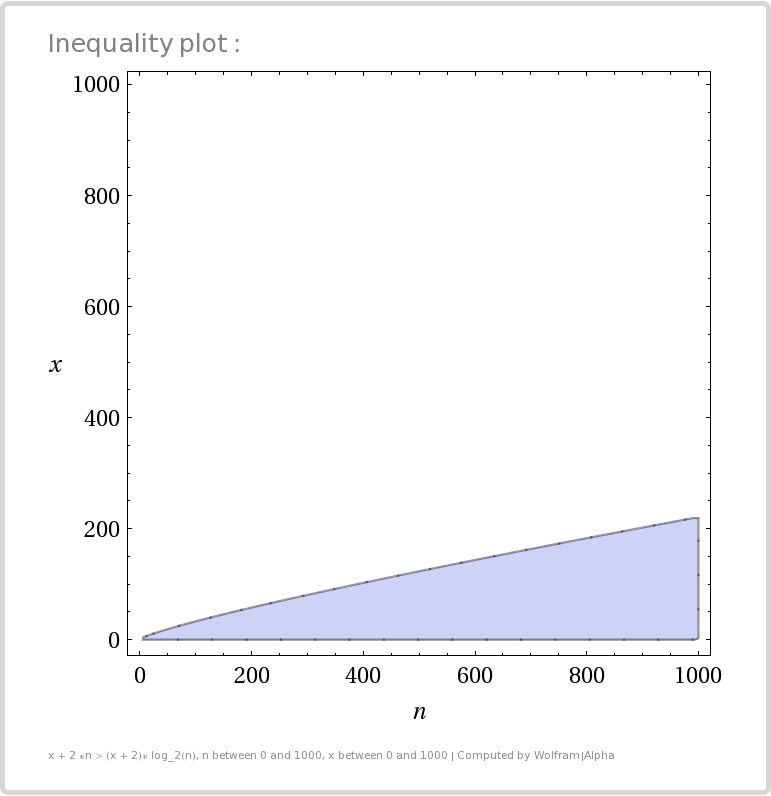
\includegraphics[width=0.7\textwidth]{thesis-pics/dsu-weight-example.png}
                \end{center}

                \caption{Plot of profitability of data structures for \autoref{fig:dsu-weight-bad-example} for different
                $n$ and $x$; blue --- Red Black Trees, white --- Hashtables}

                \label{fig:dsu-weight-bad-plot}
            \end{figure}

            This plot on \autoref{fig:dsu-weight-bad-plot} shows, where the better solution would be to use Red Black
            Trees (blue area), and where to use Hashtables (white area). The blue cone, although smaller, still covers a
            lot of cases. The earlier algorithm yields hashtables for virtually all examples here ($x > 2$), which means
            that the data structures chosen in the blue cone on the plot are not the best ones for the case.

            A better approach would be to approximate the current element count $N$ and actually evaluate the complexity
            function on the element count, multiplied by the weight, then the sum of those would be our metric of
            profitability of a data structure implementation. That would more accurately describe the cost and would be
            resistant to less-weighted operations making a big impact. We modify it as follows:

            \begin{equation} \label{data-structure-order-weights}
                d_1 <_{ds} d_2 \Leftrightarrow DSCOST(d_1, ds) \leq DSCOST(d_2, ds)
            \end{equation}

            where:

            \begin{equation}
                DSCOST(d,ds) = \sum \{OPCOST(o,c,ds) | (o,c) \in d \wedge o \in ds\}
            \end{equation}
            \begin{equation}
                OPCOST(o,c,ds) = c(N) * w(o, ds)
            \end{equation}
            \begin{equation}
                w(o, ds) \texttt{ is the weight of the operation } o \texttt{ in } ds
            \end{equation}

            This generalization invalidates the point of storing data structure complexities in a easily comparable way.
            Now we can just use any functions, that are reasonable to compute in small time, or even more complex ones
            if not using any runtime solutions like in \autoref{sec:transforming-on-line}. One could even try to
            approximate the time better than just in the big-O notation, so the actual constants would matter.

            For user guided approaches, like in \autoref{sec:pragmas}, user would have to manually specify a global
            count approximation for the cost optimization.

		\subsubsection{Profile-guided optimization} \label{sec:pgo}

			Profile-guided optimization (PGO) is a compiler optimization technique in computer programming
			to improve program runtime performance.  In contrast to traditional optimization techniques that
			solely use the source code, PGO uses the results of test runs of the instrumented program to
            optimize the final generated code \cite{Wipgo}.

            Usually the technique is used for optimizing hot loops and if statements, the binary saves logs of it
            working and the lines which are hit more, then a system-wide daemon can recompile the parts of the binary to
            make it faster for the common case.

			If the user has test data, he can run against his program, we can take advantage of that.  First
			we choose the best data structure using an unmodified method and link some library to the
			executable. Of course this doesn't have to be the best data structure possible. Then user can run the test
			suite with code coverage option, like \emph{gcov} in GCC, turned on in the compiler. This
			generates a file like the one shown in \autoref{fig:gcov}.

			\begin{figure} \label{fig:gcov}
				\lstinputlisting{thesis-pics/gcov.c}

				\centering \line(1,0){450}

				\lstinputlisting{thesis-pics/gcov.c.gcov}

				\caption{Example of a source code file and the .gcov file, generated by running the
				compiled program}

				\label{fig:gcov}
			\end{figure}


			Then the user can pass the \emph{gcov} generated files and the source code to the framework
			again. The framework can extract line hits from the \emph{gcov} files on the data structure
			operations and set weights on the operations according to the extracted data and then use the
			choosing algorithm for operations with weights from \autoref{sec:choose-weights}.

            In this method we can approximate the element count $N$ basing on our coverage data, counting all inserting
            and deleting operations.

			It's a better solution than letting the user set the weights himself, but still, the data the
			inference is based upon comes from tests and there's no guarantee the real world data will
			match the test data.

		\subsubsection{Transforming data structures on-line} \label{sec:transforming-on-line}

            Another technique known in compilers we might use is called Just-In-Time Compilation (JIT). JIT, also known
            as dynamic translation, is a method to improve the runtime performance of computer programs based on byte
            code (virtual machine code). Since byte code is interpreted it executes more slowly than compiled machine
            code, unless it is actually compiled to machine code, which could be performed before the execution – making
            the program loading slow – or during the execution. In this latter case – which is the basis for JIT
            compilation – the program is stored in memory as byte code, but the code segment currently running is
            preparatively compiled to physical machine code in order to run faster.\cite{Wijit}

            This technique is, as PGO (\autoref{sec:pgo}), used mostly for peephole optimizations, which means we always
            look at a small part of the code, like a hot if statement or a loop. With PGO we gathered information
            overtime and changed the binary, JIT does basically the same thing, only works in runtime. Usually we
            implement some proxy abstraction, that decides if, at the current time, it's profitable, to compile the
            executed part to assembly instead of interpreting it.

            Instead of compiling a bytecode to assembly, we can use a proxy to count the specific operations on our
            data structure, using the counts of usage as the new weights in the data structure inference algorithm in
            \autoref{sec:choose-weights}. We substitute the data structure with a faster one, if the program would
            obviously benefit time-wise from the substitution. New implementation could of course be compiled from a
            bytecode (e.g. LLVM IR) to assembly just like the standard JIT approach does it.

            The element count $N$ can be computed precisely, because we proxy all the data structure operations, so we
            just keep a counter.

            The heuristics for detection of a good moment for the substitution should be stronger and more careful than
            in the standard JIT way. Compiling a part of code to assembly, in most cases, isn't as costly as
            rebuilding a data structure, because unused code won't be run and a wrong data structure can slow down the
            whole program quite a bit. Building a sensible set of heuristics is very hard even for the standard JIT,
            e.g. the PyPy project tried a lot of different JIT approaches, before finding the one that is working well.
            Depending on the heuristics here, this may be the most beneficial option for a program, or a big performance
            hit.

	\subsection{Different element types}

		Currently the framework works only for integer elements. We could extend it to every primitive type in
		C, but it would require some changes.  Some data structures require the type to be comparable, which
		wouldn't be a big problem, because there is a comparison semantics defined on those types. There's also
		a hash function needed, because some data structures, like a hashtable, need to compute hash values to
		work. We can just use the binary representation of other types, and use it as an integer for the hash
		function. This whole modification doesn't need any user interaction.

		There's a bigger problem with composite types. Comparing pointers isn't obvious. You may want to compare
		addresses or the contents under that address, depending if you want object or structural equality. The
		same problem is with hash function arguments. There's also a problem with possible memory leaks. You can
		pass a pointer to a string to the data structure and lose the pointer in the program, then when the
		structure deletes the pointer and the string stays in the memory to the program's end. Adding this to
		the framework would require passing the comparison function, hash function and some kind of destructor
		function to the data structure, or possibly use some reference counting system. It would be very
		technical and would be beyond the scope of this thesis. With an array or a big struct passed to the
		framework, there's a problem if we want to share the data structure and just copy the pointer, copying
		the whole thing may be a bad idea, because it can have quite a lot of data inside.

		\subsubsection{Linked data structures}

			When we want to store structs like \autoref{fig:linked-struct} in a data structure, the
			framework, at the moment, could generate some data structure for this kind of structs. The
			operation on the data structure would look like on \autoref{fig:struct-old}.

            \begin{figure}[h!]
				\lstinputlisting{thesis-pics/linked-struct.c}

				\caption{An example record, that we want to store in a data structure}

				\label{fig:linked-struct}
			\end{figure}

            \begin{figure}[h!]
				\lstinputlisting{thesis-pics/struct-old.c}

				\caption{Use of the dsinf calls, to perform some data structure operations with the
				records; not very comfortable to use}

				\label{fig:struct-old}
			\end{figure}

			In \autoref{fig:struct-old} a comparison function is used, it compares the height. We can use
			any function that compares a coordinate or a combination of coordinates, but only one order of
			the elements is available per data structure. This can also be achieved without using structs at
			all, like in \autoref{fig:struct-pointer-sizeof-reduction}.

            \begin{figure}[h!]
				\lstinputlisting{thesis-pics/struct-pointer-sizeof-reduction.c}

				\caption{Encoding of the problem of having one order data structure on records in C,
				into code using pointers}

				\label{fig:struct-pointer-sizeof-reduction}
			\end{figure}

			In \autoref{fig:struct-pointer-sizeof-reduction} we dereference structs as arrays of
			chars. To get to any field, we just take a pointer to a field in the array and cast it to the
			right type. So it doesn't really give us any more expressiveness. It would be nice if our
			program enabled things like comparing structs by more than one condition in one program. We
			would want to be able to use operations like in \autoref{fig:struct-new}.

            \begin{figure}[h!]
				\lstinputlisting{thesis-pics/struct-new.c}

				\caption{Examples of the new dsinf API, that takes different orders on structs into
				account}

				\label{fig:struct-new}
			\end{figure}

            We change the current API of dsinf (\autoref{fig:struct-api-change}), to enable passing an arbitrary number
            of comparison functions defining orders on the data to the constructor $init\_d$. We use the $va\_args$
            mechanism in C, that's why we need the order count as the first argument, because the $va\_arg$ macro needs
            the first argument of a known type, to start iterating over the rest of the arguments. Next arguments are
            function pointers of type $int(void *, void *)$.

            \begin{figure}[h!]
				\lstinputlisting{thesis-pics/struct-api-change.c}

				\caption{Change for the API, so we can define multiple orders on data}

				\label{fig:struct-api-change}
			\end{figure}

            To achieve such thing, we need to change the way we choose structures for record types. We will check all
            the data structure tuples, of length of the order count, in the cross-product of all data structures. The
            result will be a linked data structure, i.e. a number of data structures, in which elements have pointers to
            elements in other data structures, representing the same element value --- like on
            \autoref{fig:linked-data-structures}. For example, if we have the code from the earlier example
            \autoref{fig:struct-new}, we may have a (Red-Black-Tree, Hashtable) pair, where the RBT is for the $weight$
            order, and the hashtable is for the $height$ order.

            \begin{figure}[h!]
                \begin{center}
                    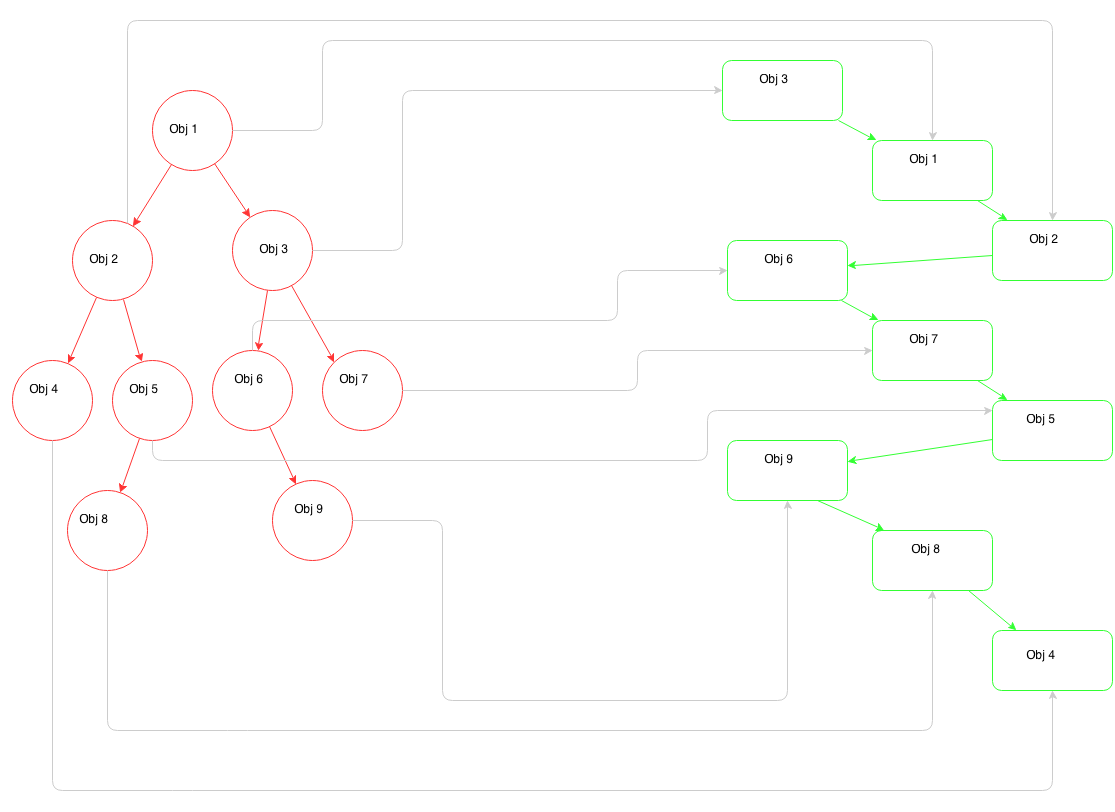
\includegraphics[width=0.9\textwidth]{thesis-pics/linked-dses.png}
                \end{center}

				\caption{Visualization of a linked data structure, elements from a balanced tree, represeting one order of data,
                 connected with the elements of a linked list, representing the second order of data}
				\label{fig:linked-data-structures}
			\end{figure}

            First we modify the $DSU()$ definition for record variables.

            In the choice algorithm we make distinctions to the operations that are order specific and general
            operations. An example of an order specific operation is $max\_d$, which finds an element that is maximal in
            the given order; an example of a general operation is $insert\_d$, which doesn't take the order as an
            argument, it has to perform an operation on both linked data structures. Sometimes order specific
            operations, aside from performing an operation on the data structure responsible for their order, they have
            to update the state in other data structures, e.g. $delete\_max\_d$ after firing has to run a $delete\_d$
            operation on the element on the other data structures responsible for different orders. It doesn't have to
            be the same operation, like in the example, $delete\_max\_d$ doesn't have to call $delete\_max\_d$, because
            it already has the data structure element pointer, and can just call $delete\_d$ --- we call the operation
            that will have the desired effect with the smallest complexity cost. For the final cost of an operation on a
            linked data structure we take the sum of costs of operations on all the data structures, which is
            big-O-wise just the most costly operation.

            \todo{Finish the rest}
            
	\subsection{Upper bound on the element count}

		When analyzing the input program, we can try to get the information, if the maximum element count in the
		data structure is bounded by some constant. If we can obtain such an information (for most programs it
		probably will be undecidable), we can use it to enhance the data structure generated for the program.

		When the element count in the data structure is potentially infinite, we have to create an
		implementation of the structure that allocates memory lazily, when it needs the space for new elements.
		We can imagine that a structure can allocate one chunk on every insertion and free a chunk on every
		deletion, or even allocate twice as big chunks and amortize the number of allocations to $O(log \; n)$.

		When we have the information about the element count, we can allocate the whole static buffer for the
		data structure, and this removes the whole cost of allocation during insertions and deletions.

		Using the technique described in \autoref{sec:transforming-on-line} we can transform our dynamic
		allocating data structure in a static one, if we are in a place in the program, from which we can't
		insert any more elements. The example on \autoref{fig:upper-bound-transform} shows such a program.

		\begin{figure}
			\lstinputlisting{thesis-pics/upper-bound-transform.c}

			\caption{An example showing a situation, where beneficial would be to transform a dynamic data
			structure into a similar structure, but with all memory statically allocated already}

			\label{fig:upper-bound-transform}
		\end{figure}

		In \autoref{fig:upper-bound-transform} after the first loop, there are no more insertions into the data
		structure, so we can mark this spot and when we the control goes to that place, we transform the data
		structure into a static version of it, allocating a big chunk of memory and deallocating all that was
		left. This way to the end of the program we won't have to do any allocations.

	\subsection{Minimal element count threshold}

		It's worth noticing that we compare only the asymptotic complexity of data structures. Some awfully
		complicated structures can have good asymptotic results, but the constant is quite high. We can avoid
		this problem by setting a threshold for each structure, what is the smallest number of elements to use
		this data structure.

		Another problem arises, how to know at compile time, how many elements a data structure will have at
		runtime. We can ask the user to explicitly specify the number during compilation or we can try to
		detect how big the declared data is, with some kind of constant folding analysis, that checks if the
		insertion to the data structure is in a loop that is run more times than the threshold. This is a fragile
		solution, because not a lot of programs are easy to analyze this way.

		Another solution is runtime tallying the size, and using the method of transforming data structures
		on-line described in \autoref{sec:transforming-on-line}. When we hit a threshold for a data structure
		with a bigger constant, but overall better fitting to our task, we transform the old one into this one.

		\begin{figure}
			\lstinputlisting{thesis-pics/minimal-elem-count.c}

			\caption{An example showing a situation, where beneficial would be to transform a data structure
				into a more complex one, because the number of elements is sufficiently big, so the
				whole transformation is profitable}

			\label{fig:minimal-elem-count}
		\end{figure}

        In \autoref{fig:minimal-elem-count} we see a code example that would yield some kind of a priority queue in our
        framework, although it only has a few elements, and some of the fastest priority queues are pretty heavy-weight
        and it would be better just to use some simpler data structure, because the setup cost isn't amortized by the
        operations.

	\subsection{Generic data structure modifications} \label{sub:gdsm}

		When searching for the most apt data structure, we need to have some kind of data structure database,
		where we keep all the structures' metadata and implementations for the framework to use. Ideally there
		would be a lot of different data structures there.

		When implementing a data structure, one could easily modify the implementation to maybe match some rare
		specific task, that is not needed in most cases. It would be wasteful to keep a copy of the data
		structure for each small combination of those modifications, if we want to return a data structure
		tailored perfectly to the task. Of course some of the modifications are very data structure specific, so
		a generalization isn't possible, but for some cases, we can extract a piece of code, like a wrapper for
        a data structure that modifies its behavior in some specific way (similar pattern was used in
        \cite{Okasaki}).

		\subsubsection{Extremal element cache}

			When we want to be able to lookup extremal elements in the data structure, we don't really have
			to know the implementation specifics of the data structure. We only need to intercept the calls
			which insert and delete elements. When we insert an element, we compare it to a cache variable,
			which keeps the biggest element (if our extremal element is the maximal element) known to be in
			the data structure.

			But this road also has some drawbacks, if we delete an element, and it occurs that the deleted
			element is the current maximum, we have to find the new maximal element from the rest of
			elements, which can be asymptoticly more costly than the delete itself.

			\missingfigure{table of cost changes}

			\begin{figure}
				\lstinputlisting{thesis-pics/elem-cache.c}

				\caption{An example implementation of the extremal element cache data structure wrapper}

				\label{fig:elem-cache}
			\end{figure}

			We notice that a lot of data structures already implement this pattern \cite{Wiveb}.

        \subsubsection{Linked elements}\label{sec:gdsm:le}

			When we have a structure that keeps some data, to find a predecessor or a successor, it usually
			takes $O(n)$ or $O(log \; n)$ operations.  To help this we can create an overlay with a doubly
			linked list on the elements, so our predecessor/successor lookups are $O(1)$. Drawback here is
			that the cost of insert is increased by searching the successor to link it appropriately.

			\begin{figure}
				\lstinputlisting{thesis-pics/linked-elements.c}

				\caption{An example implementation of the linked elements data structure wrapper}

				\label{fig:linked-cache}
			\end{figure}

\section{Future work} \label{sec:future}
	It may be a good idea to rewrite the framework to analyze LLVM\cite{LLVM} intermediate representation internally,
    instead of the C language abstract syntax tree. This could yield better results because of the optimizations that clang
    \cite{Clang} can apply to
	the initial code, like removing unnecessary calls to data structure operations, so the framework can infer the
	data structure based on the optimized code. LLVM also enables a link-time optimization, so after linking the
	chosen data structure to a program, another optimization step is performed. Also analyzing LLVM IR is easier
	than analyzing the C language.

    Framework can be easily generalized to substitute data structure comparison functions, so one could write a function
    that takes e.g. I/O into account, or any combination of I/O and big-O complexity or even something more complicated.

\newpage
\begin{appendices}
\section{Technical Documentation}
	\subsection{Compilation}
	To install \emph{dsinf} you need \emph{cabal} --- a haskell build manager. The preferred way of obtaining
	\emph{cabal} is by downloading the Haskell Platform (\href{http://www.haskell.org/platform/}{http://www.haskell.org/platform/})
	--- it has cabal bundled inside. You can also use a package manager of your favorite Linux distribution.
	
	After installing \emph{cabal}, clone the repository and build by running the following commands:
	  	\begin{lstlisting}
git clone https://github.com/alistra/data-structure-inferrer
cd data-structure-inferrer/
make dsinf
		\end{lstlisting}
	This will clone the \emph{dsinf} git repository and build the package using a \emph{cabal sandbox}.
	This can take a little while, but all the dependencies are installed locally and won't affect your 
	haskell setup in the system. This will install the \emph{dsinf} binary in your current working directory.
	\subsection{Usage}

	The program has a few modes of working:
	\begin{itemize}
		\item Recommendation mode - the framework analyzes the input files and the data structure operations in
			them, then outputs the recommended data structure on standard output
		\item Advice mode - the framework checks if any small change in the data structure operations would give
			the program a speed boost
		\item Compile mode - works as the Recommendation mode, but instead of printing the data structure to
			standard output, it compiles the files and links it with the chosen structure implementation.
	\end{itemize}
	
	We can trigger the modes using appropriate flags:
	
	\begingroup
    \fontsize{8pt}{12pt}\selectfont
    \begin{verbatim}  
% ./dsinf -h
dsinf [-OPT1 [VAL1] [-OPT2 [VAL2] [...]] [-- [CCOPTS]]
  -o file  --output=file  Output file
  -r       --recommend    Give recommendations about the data structure in the supplied code (default)
  -a       --advice       Give advice about the data structure in the supplied code
  -c       --compile      Compile the code with recommended structure linked
  -i       --inline       Inline the code implementing the recommended structure in the supplied code
  -v       --verbose      Enable verbose messages
  -h       --help         Show help

CCOPTS are passed directly to the compiler
    \end{verbatim}  
\endgroup
	
	We can run \emph{dsinf} on some test files just to check if everything is working alright.
	\begin{verbatim}
% ./dsinf C/tests/d1_delmax_d2_max.c

C/tests/d1_delmax_d2_max.c:
The recommended structure for:
d1 in main
is:
Red-Black Trees
The recommended structure for:
d2 in main
is:
Hashtable with extreme element caching
	\end{verbatim}
	
	\subsection{Implementation}
		\subsubsection{Core - Recommend.hs} \label{sec:recommend-impl}
		The core part of the recommendation engine is actually very simple:

\begin{verbatim}
recommendDS :: [OperationName] -> IO Structure
recommendDS opns =  do
    let sorted = reverse $ sortBy (\x y-> compareDS x y opns) allStructures
    let bestStructures = head $ groupBy (\x y -> compareDS x y opns == EQ) sorted
    ridx <- randomRIO (0, length bestStructures - 1)
    return $ bestStructures !! ridx
\end{verbatim}
		The argument \emph{opns :: [OperationName]} of this function is a list of data 
		structure operations performed on a persistent data structure identity in the 
		analyzed program. The \emph{allStructures} contains all the data structure definitions
		available for the recommendation engine. More about \emph{allStructures} is explained
		in \autoref{sec:all-structures-impl}. The \emph{compareDS} function is an implementation
		of the ordering in \autoref{data-structure-order}.
		
		In this functions elements from \emph{allStructures} are sorted using the \emph{compareDS} order.
		Then we take the group of first elements that are equal within this ordering --- the structures
		represent the fastest structures for the persistent data structure identity. We return a random
		fastest data structure.
		
		\subsubsection{C Analyzer - C/Analyzer.hs, Analyzer.hs}
		This part of the code uses the \emph{language-c} Haskell library to parse C code. 
		It analyzes the functions in the source files and extracts the data and passes it
		to the Core part in an easily understandable format as $DSU$s like defined in \autoref{dsu-definition}.

		To run the whole analysis, we call the \emph{analyzeC} function. It takes the file path as an argument.
\begin{verbatim}
analyzeC :: FilePath -> IO [DSInfo]
\end{verbatim}
		The return value is a list of $DSInfo$s which are just lists of $DSU$s with all the names, 
		which the particular persistent data structure identity can be called. This information is 
		sufficient to pass it to the Core described in \autoref{sec:recommend-impl}.

		The \emph{analyzeC} function traverses the whole abstract syntax tree of the program, which
		is obtained from the \emph{language-c} parser. It recurses through C statements, expressions 
		and other language parts as described in the C99 standard. It gathers the $DSU$s and groups them
		according to rules described in \autoref{dsu-definition}.
				
		\subsubsection{Data structure definitions - AllStructures.hs} \label{sec:all-structures-impl}
		This file stores all structure definitions available to the recommendation engine. 
		This is how an example definition looks like:
\begin{verbatim}
-- | Linked list
ll :: Structure
ll = DS "Linked List"       [
                            Op BoundByRef           (LinLog 1 0, N),
                            Op DecreaseValByRef     (LinLog 0 0, N),
                            Op DeleteByRef          (LinLog 0 0, N),
                            Op DeleteExtremalVal    (LinLog 1 0, N),
                            Op Difference           (LinLog 2 0, N),
                            Op Empty                (LinLog 0 0, N),
                            Op ExtremalVal          (LinLog 1 0, N),
                            Op FindByVal            (LinLog 1 0, N),
                            Op InsertVal            (LinLog 0 0, N),
                            Op Intersection         (LinLog 2 0, N),
                            Op Map                  (LinLog 1 0, N),
                            Op Size                 (LinLog 0 0, N),
                            Op SymDifference        (LinLog 2 0, N),
                            Op Union                (LinLog 0 0, N),
                            Op UpdateByRef          (LinLog 0 0, N)
                                                                    ]
\end{verbatim}
		The \emph{LinLog} constructor is stores the asymptotic complexity as described in 
		\autoref{eqn:linlog}. The \emph{N} part is a marker, that this is a normal complexity,
		as opposed to an expected or amortized complexity.
		
		This part also implements the technique described in \autoref{sub:gdsm} that provides generic 
		data structure modifications, like e.g. extremal element caching:
\begin{verbatim}
-- | A function that adds an extremal element cache to a data structure
extremalElemCache :: Structure -> Structure
extremalElemCache (DS name ops) = DS (name ++ " with extreme element caching") ops' where
    extVal = fromJust $ find (\dsop -> getOpName dsop == ExtremalVal) ops
    delByRef = fromJust $ find (\dsop -> getOpName dsop == DeleteByRef) ops
    ops' = [Op DeleteByRef (max (getComplexity extVal) (getComplexity delByRef)),
            Op ExtremalVal (LinLog 0 0, N)] ++
            filter (\dsop -> getOpName dsop `notElem` [ExtremalVal, DeleteByRef]) ops
\end{verbatim}
	The \emph{extremalElemCache} function takes a data structure definition as an input and 
	return a data structure definition with modified costs according to the generic modification.
	As adding an extremal element cache will speed up (to constant time) the lookup of an 
	extremal value, the resulting data structure definition has the cost of \emph{ExtremalVal}
	as \emph{(LinLog 0 0, N)} --- normal constant time. The tradeoff in this case is that, 
	the \emph{DeleteByRef} operation has to update the cache, if it removed the extremal value.
	Which adds the cost of the old \emph{ExtremalVal} (the new is constant) to the cost of 
	deletion.
		
		
\end{appendices}

\newpage
\begin{thebibliography}{9}
	\bibitem{Wids} Wikipedia - http://en.wikipedia.org/wiki/Data\_structure
    \bibitem{Wipgo} Wikipedia - http://en.wikipedia.org/wiki/Profile-guided\_optimization
    \bibitem{Wijit} Wikipedia - http://en.wikipedia.org/wiki/Just-in-time\_compilation
    \bibitem{Wiveb} Wikipedia - http://en.wikipedia.org/wiki/Van\_Emde\_Boas\_tree\#cite\_note-3
	\bibitem{LLVM} The LLVM Compiler Infrastructure - http://llvm.org/
	\bibitem{Okasaki} Purely Functional Data Structures - Chris Okasaki
	\bibitem{Clang} clang: a C language family frontend for LLVM - http://clang.llvm.org/
	\bibitem{AppleCC} Cocoa Core Competencies - Class Clusters - \\
		https://developer.apple.com/library/mac/\#documentation/General/Conceptual/DevPedia-CocoaCore/ClassCluster.html
\end{thebibliography}


\end{document}
% vim: set wrap tw=120:
